\chapter{Reihen}
\section{Definition und elementare Eigenschaften}

\subsection{Definition 1}

Sei $(a_n)_{n\geq p}$ eine komplexe Folge.

Das Symbol 
\[\sum_{n=p}^\infty a_n\]
ist definiert durch die Folge zugehöriger \underline{Partialsummen}
\[(S_n)_{n \geq p} \quad S_n := \sum_{j=p}^n a_j = a_p +a_{p+1} + \ldots + a_n \]
Wir nennen diese Reihe $\sum_{n=p}^\infty a_n$ konvergent, wenn die Folge der Partialsummen konvergiert und in \underline{diesem Fall} schreiben wir auch:
\[\sum_{n=p}^\infty a_n := \lim_{n\to \infty} S_n = \lim_{n\to \infty} \sum_{j=p}^n a_j\]
und nenne dieses die Summe (oder den Wert) der Reihe

\textbf{Achtung}

Damit hat das Symbol $\sum_{n=p}^\infty a_n$ zwei Bedeutungen:

\begin{enumerate}
  \item Symbol für die Folge der Partialsummen
  \item Symbol für den Grenzwert $\lim S_n$ falls diese existiert
\end{enumerate}

\begin{example}

  \begin{itemize}
    \item Beispiel einer simplen Teleskopreihe
      \[\text{Die Reihe } \sumOI \frac{1}{n(n+1)} \text{ konvergiert}\]
      \[S_n = \sum_{j=1}^n \frac{1}{j(j+1)}, \quad \frac{1}{j(j+1)} = \frac{1}{j}-\frac{1}{j+1}\]
      \[= \sum_{j=1}^n \left( \frac{1}{j}-\frac{1}{j+1} \right) = \left( \frac{1}{1}-\frac{1}{2} \right) + \left( \frac{1}{2}-\frac{1}{3} \right) + \ldots \left( \frac{1}{n}-\frac{1}{n+1} \right) \]   
      \[= 1 - \frac{1}{n+1} \text{ Teleskopreihe! }\]
      \[\implies \lim_{n \to \infty} S_n = \lim_{n\to \infty} \left(1- \frac{1}{n+1} \right) =1\]
      \[\sum_{j=1}^n \left( \frac{1}{j} - \frac{1}{n+1} \right)  = \sum_{j=1}^n \frac{1}{j} - \sum_{j=1}^n \frac{1}{j+1}\]
      \[= \frac{1}{1} - \frac{1}{n+1} = 1-\frac{1}{n+1}\]
    \item Geometrische Reihe 
     \[ \sumNI x^n
       \begin{array}{l}
         \text{ konvergiert für } |x| < 1 \\
         \text{ divergiert für } |x| \geq 1   
       \end{array}       
     \]
     
     \begin{proof}
       \[S_n = \sum_{j=0}^n x^j = \frac{1-x^{n+1}}{1-x} \text{ geometrische Summe } x \neq 1\]
       \[\text{Falls } |x|<1 \implies \lim_{n\to \infty} x^{n+1} = 0 \]
       \[\implies \lim_{n \to \infty} S_n = \lim_{n \to \infty} \frac{1-x^{n+1}}{1-x}=\frac{1}{1-x}\]
       Zur Erinnerung:
       \[x S_n = x \sum_{j=0}^n x^j = \sum_{j=0}^n x^{j+1} = \sum_{j=1}^{n+1} x^{j}\]
       \[\implies S_n-x S_n = \sum_{j=0}^n x^j - \sum_{j=1}^{n+1} x^{j} = 1 - x^{n+1}\]
     \end{proof}
  \end{itemize}

\end{example}

\subsection{Cauchy-Kriterium}

\[\text{Eine Folge } (S_n)_n \text{ konvergiert} \]
\[\Longleftrightarrow \forall \epsilon > 0 \exists k_\epsilon : |S_m -S_n|<\epsilon \quad \forall n,m \geq k_\epsilon\] 
\[m=n+l\]
\[\implies S_m - S_n = S_{n+l} - S_n = \sum_{j=p}^{n+l} a_j -\sum_{j=p}^n a_j = \sum_{j=n+1}^{n+l} a_j\]

\subsection{Satz 2: Cauchy-Kriterium für Konvergenz von Reihen}

\[\text{Eine Reihe } \sum_{n=p}^\infty a_n \text{ konvergiert} \]
\[\Longleftrightarrow \forall \epsilon > 0 \exists k_\epsilon : \forall l \in \N, n \geq k_\epsilon : \left|\sum_{j=p}^{n+1} a_j\right|<\epsilon\]


\begin{proof}
  \[\sum_{n=p}^\infty a_n \text{ konvergiert } \Longleftrightarrow \text{ die Folge } (a_n)_{n\geq p} \text{ der Partialsummen konvergiert}\]
  \[\stackrel{\text{Cauchy-Krit}}{\Longleftrightarrow} \forall \epsilon > 0 \exists k_\epsilon : | S_m -S_n | < \epsilon \quad \forall n,m \geq k_\epsilon\]
  \[\text{O.B.d.A } m>n \text{ d.h. } m=n+l,l\in \N\]
  \[\text{da } S_m-S_n = S_{n+l}- S_n = \sum_{j=n+1}^{n+l} a_j \text{ sind wir fertig}\]

\end{proof}

\subsection{Korollar 3}

\[\text{Wenn } \sum_{n=p}^\infty a_n \text{ konvergiert, dann ist } (a_n)_{n \geq p} \text{ eine Nullfolge} \]
\[\text{d.h. } \lim_{n\to \infty} a_n = 0\]
\textbf{Bemerkung}
Umkehrung gilt NICHT!

\[\text{z.B. die harmonische Reihe } \sumOI \frac{1}{n} \text{ divergiert}\]

\begin{proof}
  \[\text{Wende } \mqq{\implies} \text{ Richtung auf } l=1 \text{ an}\]
  \[\sum_{n=p}^\infty a_n \text{ konvergiert } \implies \forall \epsilon > 0 \exists k_\epsilon : \underbrace{\left| \sum_{j=n+1}^{n+1} \right|}_{|a_{n+1}}<\epsilon\]
  \[\text{d.h. } a_{n+1} \to 0\]
  \[\text{d.h. } a_{n} \to 0\]
\end{proof}

\begin{proof} (Anderer Beweis)
  \[S_n = \sum_{j=0}^n a_j, \quad n \geq p\]
  \[\lim_{n\to \infty} S_n = L\]
  \[a_n = S_n - S_{n-1}\]
  \begin{align*}
    \implies \lim_{n\to \infty} a_n & = \lim_{n_\to \infty} (S_n - S_{n-1}) \\
                                    & = \lim_{n_\to \infty} S_n - \lim_{n_\to \infty} S_{n-1} \\
                                    & = L-L = 0
  \end{align*}
 
\end{proof}

\subsection{Korollar 4: Die harmonische Reihe ist divergent}

\[\sumOI \frac{1}{n} \text{ divergiert}\]

\begin{proof}
  
  \[\text{Wen sie konvergent wäre, dann gilt Satz 2 }\] 
  \[a_n = \frac{1}{n} , S_n = \sum_{j=1}^n a_j = \sum_{j=1}^n \frac{1}{j}\]
  \[l=n\]
  \[S_{n+l}-S_n = \sum_{j=n+1}^{n+n} \frac{1}{j} = \sum_{j=n+1}^{2n} \frac{1}{j} = \frac{1}{n+1} + \frac{1}{n+2} + \frac{1}{n+3} + \ldots + \frac{1}{2n} \geq n*\frac{1}{2n}=\frac{1}{2}\]
  d.h. Satz 2 ist verletzt $\implies$ keine Konvergenz
\end{proof}

\subsection{Satz 5}

\begin{enumerate}
  \item (Verschiebung des Summantenanfangs)
  
  Sei $(a_n)_{n \geq p}$ eine Folge, $b_j = a_{p+j}, j \in \N_0$
  
  Die Reihe $\sum_{n=p}^\infty a_n$, $\sum_{j=0}^\infty b_j$ und $\sum_{n=q}^\infty a_n$. Für $p < q$, haben dasselbe Konvergenzverhalten (d.h. sind gleichzeitig konvergent oder bestimmt divergent oder divergent) und im Falle der Konvergenz gilt:
  \[\sum_{j=0}^\infty a_{p+j} = \sum_{n=p}^\infty a_n = a_p + a_{p+1} + \ldots + a_{q-1} + \sum_{n=q}^\infty a_n \]
  
  \begin{proof}
    \[\text{Sei } S_n = a_p + a_{p+1} + \ldots + a_n\]
    \[t_n = a_q + a_{q+1} + \ldots + a_n,n > p\]
    \[U_n = b_0 + b_1 + \ldots + b_n\]
    \[A = a_p+ \ldots + a_{q-1}\]
    \[\implies S_n = A+ t_n, n\geq q\]
    \[\implies (S_n)_{n\geq p} \text{ konvergiert } (t_n)_{n\geq q} \text{ konvergiert und } \lim_{n\to \infty} S_n = A + \lim_{n\to \infty} t_n\]
    \begin{proof}
      \[\text{Wegen 1) reicht es Reihen der Form } \sumOI a_n \text{ zu betrachten} \]
    \end{proof}
  \end{proof}  
  
  \item Das Konvergenzverhalten einer Reihe ändert sich nicht, wenn wir endlich viele Terme weglassen oder hinzufügen.
  
  \begin{proof}
    \[\text{Folgt aus 1)}\]
  \end{proof}    
  
  \item Sei $(g(k))_{k=1}^q$ die endliche $(q<\infty)$ oder unendliche $(q=\infty)$ Indexfolge mit $1\leq g(1) < g(2) < \ldots < g(k) < g(k+1)$
  
  $g(k)\in \N$ und $a_j=0$, wenn $j \neq g(k) \quad \forall k \in \N$
  
  (d.h. $a_j \neq 0 \Longleftrightarrow \exists k \in \N: j=g(k)$)
  
  Dann haben die beiden Reihen $\sumOI a_n$ und $\sum_{k=1}^\infty a_{g(k)}$ dasselbe Konvergenzverhalten.
  
  (D.h. in einer Reihe kann man Nullen beliebig weglassen oder hinzufügen)
  
  \begin{proof}
    \[\text{Sei } S_n=\sum_{l=1}^n q_l, t_n = \sum_{j=1}^n a_{g(j)}\]
    \[\text{ist } q<\infty \implies S_n = t_n \forall n \geq g(q)\]
    \[\text{ist } q=\infty \text{ dann ist } \boxed{S_n =t_n \text{ für } g(k)\leq n< g(k+1)}\]
    \[\text{Also konvergiert } S_n \Longleftrightarrow t_n \text{ konvergiert und } \lim_{n\to \infty} S_n = \lim_{n \to \infty} t_n\]
  \end{proof}
\end{enumerate}

\subsection{Satz 6}

\[\text{Sind } \sumOI a_n, \sumOI b_n \text{  konvergiert, so ist } \forall \lambda, \mu \in \mathbb{C}\]
\[\sumOI (\lambda a_n + \mu b_n) \text{ konvergiert  und } \sumOI (\lambda a_n + \mu b_n) = \lambda \sumOI a_n + \mu \sumOI b_n \]

\begin{proof}
  \[S_n = \sum_{l=1}^n a_l \to s\]
  \[t_n = \sum_{l=1}^n b_l \to t\]
  \[\implies \sum_{l=1}^n (\lambda a_l + \mu b_l) = \lambda S_n + \mu t_n \to \lambda s + \mu t\]
\end{proof}

\subsection{Korollar 7}

\[\text{Aus der Konvergenz von } \sumOI a_2n, \sumOI a_{2n+1}\]
\[\text{folgt die Konvergenz } \sumOI a_n
\text{ und } \sumOI a_n = \sumOI a_{2n} + \sumOI a_{2n+1}\]

\begin{proof}
  \[\text{Man fülle die Teilreihen } \sumOI a_{2n} \text{ und } \sumNI a_{n+1}\]
  \[\text{mit Nullen auf (vergleich Satz 5 3)) und wende die Additionsregel Satz 6 an}\] 
\end{proof}

\underline{Warnung:} Umkehrung gilt NICHT! (Bsp. später)

\section{Alternierende Reihen}

Sei $(b_n)_n$ eine Nullfolge, $b_n \geq 0$. Dann wird
\[\sumOI (-1)^{n-1} b_n\]
Eine alternierende Reihe genannt!
\[S_n = \sum_{j=1}^\infty (-1)^{j-1} b_j = b_1-b_2+b_3-b_4+\ldots+(-1)^{n-1} b_n\]

\[\text{z.B.: } \sumOI (-1)^{n-1} \frac{1}{n}\]

\subsection{Satz 8: Leibniz-Konvergenzkriterium}

Sei $(b_n)_n$ eine fallende Nullfolge d.h. $b_n \to 0$ und $b_n \geq b_{n_1} \quad \forall n \in \N$ 

dann konvergiert die alternierende Reihe
\[\sumOI (-1)^{n-1} b_n = b_1-b_2+b_3-b_4+\ldots \]

\begin{proof}
 \[\text{Aus } b_n \geq b_{n+1} \to 0\]
 \[\implies b_n \geq 0 \quad \forall n\]
 \[S_{2k}:=\sum_{n=1}^{2k} (-1)^{n-1} b_n = \underbrace{(b_1-b_2)}_{\geq 0}+\underbrace{(b_3-b_4)}_{\geq 0}+\ldots+\underbrace{(b_{2k-1}-b_{2k})}_{\geq 0}\]
 \[S_{2k+1}:=\sum_{n=1}^{2k+1} (-1)^{n-1} b_n = b_1 - \underbrace{(b_2-b_3)}_{\geq 0}-\underbrace{(b_4-b_5)}_{\geq 0}-\ldots-\underbrace{(b_{2k}-b_{2k+1})}_{\geq 0}\]
 \[\implies S_{2k} \text{ ist wachsend, } S_{2k+1} \text{ ist fallend}\]
 \[\text{d.h. } S_{2k} \leq S_{2(k+1)} = S_{2k+2}, S_{2k+1} \geq S_{2(k+1)+1} = S_{2k+3}\]
 \[\text{und } 0\leq S_{2k} \leq S_{2k+1} \leq b_1\]
 \[\stackrel{\begin{array}{l}\text{Monotone}\\\text{Konvergenz}\end{array}}{\implies} \lim_{k \to \infty} S_{2k}, \lim_{k \to \infty} S_{2k+1} \text{ existieren} \]
 \[\text{Außerdem gilt: } |S_{2k+1}-S_{2k}|=b_{2k+1} \to 0\]
 \[\text{Somit ist } \lim_{n\to \infty} S_{2k+1} = \lim_{n\to \infty} S_{2k} = s\]
 \[\implies \lim_{n \to \infty} \sumOI (-1)^{n-1} b_n=s\] 
\end{proof}

\subsection{Ultimative Version von Leibniz}
Frage $\sum_{n=0}^{\infty} a_n \cdot b_n \hspace{10mm} b_n > b_{n+1} \to 0$ wann konvergiert das? \\
Antwort: Oszillationen in den $a_n$ helfen!

z.B. $a_n = (-1)^{n+1} \implies a_1 = 1 \hspace{5mm} a_2 = -1 \ldots $
$$A_n = \sum_j=n^{n} a_j = 1-1+1-1+1-1 \ldots =  
\begin{cases}
\text{1 wenn n ungerade}	\\
\text{0 ansonsten }		\\
\end{cases}
$$

$A_n$ ist eine beschränkte Folge

\subsection{Satz 9 (Ultimativer Leibniz)}
Sei $(a_n)_n \in \mathbb{C} (b_n)_n \in \R$ mit $b_n \geq b_{n+1} \lim_{n \to \infty} b_{n} = 0 $ und $sup | \sum_{j=1}^{n} a_j| < \infty$
$\implies  \sumOI a_n b_n konvergiert$

\begin{proof}
 Zu zeigen(nach Cauchy) $\forall \epsilon > 0 \hspace{5mm} \exists k_\epsilon: \forall l \in \N, n \ge k_\epsilon:$
 $$| \sum_{j=n+1}^{n+l} a_j b_j | < \epsilon$$
 
 \begin{equation}
  \begin{split}
    \text{Setzen } & A_n := \sum_{j=1}^{n}a_j, A_0 = 0 \\
    & \implies a_j = A_j - A_{j-1} \\
    & \implies \sum_{j=n+1}^{n+l}  a_j b_j = \sum_{j=n+1}^{n+l} (A_j - A_{j-1}) b_j \\
    & = \sum_{j=n+1}^{n+l}  A_j b_j - \underbrace{\sum_{j=n+1}^{n+l}  A_{j-1} b_j}_{= \sum_{j=n}^{n+l-1} A_j b_{j+1}} \\
    & = A_{n+l} b_{n+l} = A_n b_{n+l} + \sum_{j=n+1}^{n+l-1} A_j (b_j - b_{j-1}) \\
    & \implies | \sum_{j=n+1}^{n+l}  a_j b_j | \le | A_{n+1} | b_{n+l} + |A_n| b_{n+1} + \sum_{j=n+1}^{n+l-1} |a_j| |b_j - b_{j+1}|  \\
    & M := sign(Ai) < \infty \le M (b_{n+l} + b_{n+1}) + M \sum_{j=n+1}^{n+l+11} (b_j - b_{j+1})  \text{  da  } b_j > b_{j+1} \\
    & \implies |\sum_{j=n+1}^{n+l} a_j b_j| \le M(b_{n+l} + b_{n+1}) + M (b_{n+l} - b_{n+l}) \\
    & = 2 M(b_{n+1}) \to 0 \\
    & \text{unabhängig von l!}
  \end{split}
 \end{equation}
\end{proof}

Bsp: $z \in \mathbb{C} \hspace{5mm}  |z| = 1 \hspace{5mm} z \neq 1$
$b_n $ fallende Nullfolge
$\sum z^{n-1} b_n$ konvergiert

\begin{equation}
 \begin{split}
  A_n & := \sum_{j=1}^{n} z^{j+1} = \sum_{j=0}^{n+1}z^j = \frac{1-z^n}{1-z} \\
  |A_n| & = |\frac{1-z^n}{1-z}| = \frac{1}{|1-z|} | 1-z^n| \leq \frac{1}{|1-z|}
  \cdot (1+|z|^n) = \frac{z}{|1-z|}
 \end{split}
\end{equation}

\section{Monotone Reihen}
Sei $(a_n)_n \in \R, a_n > 0$ \\
$\rightsquigarrow s_n = \sum_{j=1}^n a_j$ ist wachsend!
%TODO: Verweis einfügen
also nach Satz von der monotonen Konvergenz
Konvergenz $(s_n)_n \Leftrightarrow s_n$ beschränkt

\subsection{Satz 10}
  \begin{equation}
    \begin{split}
      \text{Eine Reihe} \sumOI a_n a_n>0 \text{konvergiert} \\
      \Leftrightarrow \exists k < \infty : \sum a_j < k \forall n \in \N
    \end{split}
  \end{equation}
  \begin{proof}
    \begin{equation}
      \begin{split}
	s_n \le s_{n+1} \forall n \\
	\implies \sum a_n &= sup s_n = sup \sum_{j=1}^{n} a_j \\
	\text{setzen }sup_n &= -\infty \text{falls Folge nicht beschränkt ist} \\
	\implies \sumOI a_n = sup s_n a_n \ge 0
      \end{split}
    \end{equation}
  \end{proof}

\subsection{Korollar 11}
  Für $\sumOI a_n $ , $a_n \ge 0$ gilt entweder
  \begin{itemize}
    \item $\sum_{n+1}^{\infty} a_n \le \infty$
    \item $\sum_{n+1}^{\infty} a_n \ge \infty$
  \end{itemize}
  Erstens bed. $s_n$ konvergent, letztes $s_n$ divergiert gegen $\infty$

\subsection{Satz 12}
Ist $o \le a_n \le b_n \forall n$ und $\sumOI b_n$ konvergiert \\
$ \implies \sumOI a_n$ konvergiert und $ \sum a_n \le \sum b_n$ \\
\begin{proof}
 \begin{equation}
  \begin{split}
    s_n := \sum_{j+1}^n a_j und t_n := \sum_{j+1}^n b_j \\
    \implies s_n \le s_{n+1} t_n \le t_{n+1} \\
    s_n < t_n \forall n 
    \text{Falls} t_n \to r \in \R n \to \infty \\
    \implies r = sup t_n \\
    \implies s_n \le \underbrace{sup t_k}_{k \in \N} \in \R \\
    \implies (s_n)_n \text{ist beschränkt wachsend} \\
    %TODO: Unter folgendem Pfeil mon. Konvergenz schreiben
    \implies s_n \text{ ist konvergent} \\
    \implies \sum_{n+1}^n a_n \text{ist konvergent} \\
    \text{und} \lim s_n \le \lim t_n \\
    \implies \sumOI a_n \le \sumOI t_n
   \end{split}
 \end{equation}
\end{proof}

\subsection{Satz 13: Cauchyscher Verdichtungssatz}
Sei $(a_n)_n$ fallende Nullfolge
\begin{equation}
 \text{Dann ist } \sumOI a_n \text{konvergent} \Leftrightarrow \sumOI 2^n a_{2n} \text{konvergent}
\end{equation}

\begin{proof}
 \begin{equation}
  \begin{split}
   s_j & := \sumOI a_n t_j := \sumOI 2^n a_2n \\
   & ln  j \le 2^k \text{gilt} (a_n \ge a_n+1) \forall n \\
   s_j &= a_0 + a_1 + \underbrace{a_2 + a_3}_{\le 2a_2} + a_4 + \ldots + (a_{2^k} + a_{2^(k+1)} + \ldots + a_{2^{k+1}-1}) \\
   & \le a_0 + a_1 + 2a_2 + 4 a_4 + 8 a_8 + \ldots + 2^k a_{2^k} \\
   & =t_k \le t_{k+1} \le \ldots \le t_{k+l} \forall l \in \N \\
   & \implies s_j \le \underbrace{sup(t_k) < \infty}_{\text{wenn kondensierte Reihe konvergent}} \\
   & \implies s_j \text{ konvergiert}
  \end{split}
 \end{equation}
Umkehrung ähnlich zu zeigen.
\end{proof}
\subsection{Anwendungen des Cauchyschen Verdichtungskriteriums}
\begin{itemize}
 \item $\sumOI \frac{1}{n}$ divergiert
 \item $\sum_{n\le1}^{\infty} 2^n \frac{1}{2^n} = \sumOI 1$ divergent
 \item $\sumOI \frac{1}{\lambda} $ konvergiert $\lambda > |1|$ divergiert $\lambda \le |1|$
\end{itemize}

\section{Absolut konvergente Reihen}
hier auch $(a_n)_n \in \mathbb{C}$
\subsection{Def 14}
Eine Reihe $\sumOI a_n$ konvergiert absolut, wenn die Reihe $\sumOI |a_n| $ konvergiert.

\subsection{Satz 15}
Eine absolut konvergente Reihe $\sumOI a_n$ ist 
\begin{itemize}
 \item konvergent
 \item es gilt: $|\sumOI a_n| \le \sumOI |a_n| $
\end{itemize}
\begin{proof}
  $|\sum_{j\geq n+1}^{n+l} |a_j| < \epsilon$\\
  $\forall \epsilon > 0 \exists k_\epsilon : \sum_{j=n+1}^{n+l} |a_j| < \epsilon , \forall l \in \mathbb{N}, n \geq k_\epsilon$\\
  $\implies \sumOI a_n$ ist konvergent und $|\underbrace{\sum_{j=1}^n a_j}_{\leftarrow |\sum_{j=1}^\infty a_j|, n\leftarrow \infty}| \leq \sum_{j=1}^n |a_j| \leq \sum_{j=1}^\infty |a_j|$
\end{proof}

\paragraph{Bemerkung} Umkehrung gilt nicht!\\
$\sumOI (-1)^{n-1} \frac{1}{n}$ konvergiert, aber $\sumOI \frac{1}{n} = \infty$

\subsection{Def 16}
Eine Reihe $ \sumOI c_n c_N > 0$ heißt Majorante $\sumOI a_n$, falls ein $n_0 \in \N$ existiert:
$$|a_n| \le n n>n_0 \text{d.h. falls} |a_n| \le c_n \forall n \in \N$$

\subsection{Satz 17 Majorantenkriterium}
\begin{enumerate}
 \item Hat die Reihe $\sumOI a_n$ eine konvergente Majorante so ist sie absolut konvergent und damit konvergent.
 \item Ist $a_n \ge 0$ und dazu $\sumOI a_n$ so divergiert auch jede Majorante.
\end{enumerate}

\begin{proof}
Teil 2: Selber überlegen\\
Zu 1) o.B.d.A. $|a_n| \leq a_n, \forall n \in\mathbb{N}, \sumOI c_n < \infty$\\
$\implies sum_{n=1}^\infty |a_n| \leq \sumOI c_n < \infty$\\
$\implies \sumOI a_n$ absolut konvergent und somit konvergent nach Satz 15.
\end{proof}


\subsection{Satz 18 Wurzelkriterium}
Sei $\sumOI a_n$ eine Reihe und $0 < q < 1$
mit $\sqrt[n]{|a_n|} = | a_n| \le q \text{für fast alle n}$
$$\implies \sumOI a_n \text{ist abs. konvergent}$$

\begin{proof}
  $\sqrt[n]{|a_n|} \leq q \implies |a_n| \leq q^n$ für $n \geq n_0$\\
  $\implies \sumOI a_n$ hat die konvergierende Majorante $\sumOI a^n$ da $q < 1$!\\
  Ist $\sqrt[n]{|a_n|} \geq 1$ für unendlich viele n\\
  $\implies |a_n| \geq 1 = 1$ für unendlich viele n\\
  $\implies (a_n)_n$ ist keine Nullfolge $\implies \sum a_n$ ist nicht konvergent.
\end{proof}

\subsection{Satz 19 Quotientenkriterium}
Ist $a_n \ne 0 \forall n$ und es existiert $a,b < q < 1$
mit $ | \frac{a_{n+1}}{a_n} | \le q $ für fast alle n
$$\implies \sumOI a_n \text{ist abs. konvergent}$$
mit $ | \frac{a_{n+1}}{a_n} | \ge 1 $ für fast alle n
$$\sumOI a_n \text{ist divergent}$$

\begin{proof}
Sei $|\frac{a_{n+1}}{a_n}| \leq q, n \geq n_0$\\
$l \in \mathbb{N}: |\frac{a_{n+1}}{a_n}| = \prod_{j=0}^{l-1} \underbrace{|\frac{a_{n+1}}{a_n}|}_{\leq q} \leq q^l$\\
$\implies |a_{n_0 + l}| \leq |a_{n_0}|a^l = |a_{n_0}|q^{-n_0} * q^{n_0 + l}$\\
$\implies \forall n \geq n_0: |a_n| \leq k q^n k = |a_{n_0}| q^{-n_0}$\\
$\implies \sumOI a_n$ hat die konvergente Majorante $\sumOI k q^n$!\\
Ist $|\frac{a_{n+1}}{a_n}| \geq 1$ für fast alle n\\
$\implies \underbrace{|a_{n+!}|}_{\leq |a_{n+2}| \implies |a_n| \geq |a_{n_0}|, \forall n\geq n_0} \geq |a_n|, n \geq n_0$\\
$\implies (a_n)_n$ ist keine Nullfolge!
\end{proof}
\paragraph{Bemerkung}
\begin{enumerate}[1)]
  \item Für Konvergenz reicht nicht $\sqrt[n]{|a_n|} < 1$ oder $|\frac{a_{n+1}}{a_n}| < 1$ für fast alle n. Siehe harmonische Reihe
  \item Andere Formulierung
\begin{enumerate}[a)]
  \item Die Reihe $\sum a_n$ ist absolut konvergent, wenn $\limsup_{n\rightarrow\infty} \sqrt[n]{|a_n|} < 1$, bzw. divergent, wenn $\limsup_{n\rightarrow\infty} \sqrt[n]{|a_n|} > 1$
  \item Die Reihe $\sumOI a_n$ ist absolut konvergent, wenn $\limsup_{n\rightarrow\infty} |\frac{a_{n+1}}{a_n}| < 1$, bzw. divergent falls $\lim_{n\rightarrow\infty} |\frac{a_{n+1}}{a_n}| > 1$
\end{enumerate}
\end{enumerate}
\paragraph{Beispiel}$ $\\
$a_n = \frac{1}{n^2}$:$\lim_{n\rightarrow\infty} \frac{a_{n+1}}{a_n} = 1, \lim_{n\rightarrow\infty} \sqrt[n]{n^2} = 1$\\
$\sumOI n^px^n$ konvergiert absolut $|x|<1$ nach Wurzelkriterium.\\
$\sumOI \frac{1}{n^\gamma}$ machen weder Quotienten noch das Wurzelkriterium eine Aussage.
%%ENDE Vorlesung 28.11

\section{Dezimaldarstellung reeller Zahlen}
$r\in\mathbb{R}:\lfloor r \rfloor :=$ ganzzahliger Anzahl\\
$r\in\mathbb{R}:\lfloor r \rfloor :=$ max$\{h\in\mathbb{Z}, n \leq r\}$ (Gaußklammer)\\
$x := r - \lfloor r \rfloor \in [0,1)$\\
$r = \lfloor r \rfloor + x$\\
$x_1 := \lfloor x * 10 \rfloor \in \{0,1,2,3,4,5,6,7,8,9\}$\\
$R_1 := x - x_1 * 10^{-1} \in [0,10^{-1})$\\
$x=x_1*10^{-1} + R_1$\\
$x_2 := \lfloor R_1 * 10^2 \rfloor \in \{0,1,\ldots ,9\}$\\
$x = x_1 * 10^{-1} + x_2 * 10^{-2} + R_2$\\
induktiv, wenn $x = x_1 * 10^{-1} + x_2 * 10^{-2} + \ldots + x_n * 10^{-n} + R_n$\\
$x_j \in \{0,1,\ldots,9\}, R_n \in [0,10^{-(n)})$\\
$x_{n+1} = \lfloor R_n * 10^{n+1} \rfloor$\\
$\implies x=\sum_{j=1}^{n+1} x_j * 10^{-j} + R_{n+1}, R_{n+1} \in [0,10^{-(n+1)})$\\
$\sumOI x_n 10^{-n}$ ist absolut konvergent und $x=\sumOI x_n * 1-^{-n}$\\
$\implies r = \lfloor r \rfloor + x = m,x_1,x_2,x_3,\ldots$\\
$m = \lfloor r \rfloor$\\
$r = m + \sumOI x_n * 10^{-n}$\\
$0,\overline{9} = \sumOI	9 * 10^{-n} = 9 * 10^{-1} * \sum_{k=0}^\infty 10^{-k}$ (geometrische Reihe)\\
$0,\overline{9} = 9 * 10^{-1} * \frac{1}{1-\frac{1}{10}} = 9 * 1-^{-1} * \frac{10}{10-1} = 1$!\\
Falls es ein $l \geq 1$ gibt mit $x_n = 9, \forall n \geq l + 1$. Damit ohne Darstellung nicht eindeutig! Sei l die kleinste solche Zahle $n\in\mathbb{N}_0$\\
$\implies \sum_{n=l+1}^\infty 9 * 10^{-n} = 9 * \sum_{n=l+1}^\infty 10^{-n} = 9 * 10 ^{-(l+1)} \sumNI 10^{-n} = 9 * 10^{-(l+1)} \frac{1}{1-\frac{1}{10}} = 10^{-l}$\\
$\implies x = r - \lfloor r \rfloor = \sumOI x_n * 10^{-n} = \sum_{n=1}^l x_n * 10^{-n} + \underbrace{\sum_{n=l+1}^\infty 9 * 10^{-n}}_{=10^{-l}}$\\
$=\sum_{n=1}^{l-1} x_n * 10^{-n} + \underbrace{x_l 10^{-l} + 10^{-l}}_{=(x_l + 1) * 10^{-l}}$\\
$\implies r = \lfloor r \rfloor + \sum_{n=1}^l \tilde{x}_1 * 10^{-n}$\\
$\tilde{x} = \left\{\begin{array}{cl} x_n, & \mbox{falls } n\leq l -1\\ x_l + 1, & \mbox{falls } n = l\\ 0 & \mbox{falls } n\geq l + 1 \end{array}\right. $\\
Vollkommen analog kann man g-adische Darstellung zeigen: $g \in\mathbb{N}$\\
$\implies r = m + \sumOI	y_n g^{-n}$\\
$m\in\mathbb{Z}, y_n \in\{ 0,1,\ldots ,g-1\}$\\
\begin{proof}
Analog
\end{proof}

\paragraph{Angenommen} $[0,1)$ ist abzählbar
\begin{equation}
\begin{split}
  \rightarrow \text{Liste} r_n \in [0,1), n\in \N \\
  r_1 &= 0, x_1^1, x_2^1, x_3^1, \text{ }\ldots \\
  r_2 &= 0, x_1^2, x_2^2, \text{ }\ldots \\
  r_3 &= 0, x_1^3, \text{ }\ldots \\
  \vdots
\end{split}
\end{equation}


Idee als n-te Ziffer $\tilde{x}_n := \left\{\begin{array}{cl} \tilde{x}_n + 1, & \mbox{falls } x_n^n \leq 8\\ 1, & \mbox{falls } x_n^n = 9 \end{array}\right. $\\
$\implies$ neue reelle Zahl $\tilde{r} = 0, \tilde{x}_1, \tilde{x}_2, \tilde{x}_3, \ldots \in [0,1)$ die nicht in obiger Liste ist.
$\implies [0,1)$ nicht abzählbar!

\section{Umordnung von Reihen}
\paragraph{Beobachtung} Bei \underline{endlichen} Summen hängt der Wer der Summe \underline{nicht} davon ab, in welcher Reihenfolge die Summanden aufsummiert werden.\\
$a_1 + a_2 + \ldots + a_6 = ((((a_1+a_2)+a_5)+a_4)+a_6)+a_3 = ((((a_1+a_6)+a_4)+a_3)+a_5)+a_2$

\paragraph{Warnung} Bei unendlichen Reihen ist dies manchmal falsch!

\subsection{Definition 20}
\begin{enumerate}[1)]
  \item Seien $a_n, b_n \in\mathbb{C}$
    Wir nennen $\sumOI b_n$ eine Umordnung von $\sum_P{n=1}^\infty a_n$, wenn es eine bijektive Abbildung 
    $\sigma : \N \rightarrow \N$ gibt $b_n = a_{\sigma (n)}$, d.h. $(b_n)_n$ ist eine Umordnung von $(a_n)_n$
  \item EIen konvergente Reihe $\sumOI a_n, a_n \in\mathbb{C}$ heißt unbedingt konvergent, wenn jede Umordnung $\sum_n b_n$ ebenfalls konvergent und dieselbe Summe wie $\sumOI a_n$ benutzt. Anderfalls heißt $\sum_n a_n$ bedingt konvergent.
\end{enumerate}
\subsection{Satz 21 (Dirchlet 1837)}
$a_n \in\mathbb{C}, \sumOI a_n$ ist unbedingt konvergent $\Leftrightarrow \sumOI a_n$ ist absolut konvergent!\\
\begin{proof}
\begin{enumerate}[1)]
  \item "$\Leftarrow$": \\
  Sei $\sumOI$ absolut konvergent und $\sumOI b_n$ eine Umordnung.
  $s_n := \sum_{j=1}^n a_j, t_n := \sum_{k=1}^n b_k = \sum_{k=1}^n a_{\sigma (k)}$\\
  $\sigma : \mathbb{N} \rightarrow \mathbb{N}$ Bijektion\\
  Wissen $s_n \rightarrow s,$ müssen zeigen $t_n \rightarrow s$\\
  Seien $\epsilon > 0, \implies \exists m \in \N$
  $$\sum_{n=m+1}^{m+l} |a_n| < \epsilon, \forall l \in\mathbb{N}\text{(\textasteriskcentered )}$$
  $$\text{da} \sum a_n \text{absolut konvergiert}$$

  Bestimme $N \in \mathbb{N}$ so, dass\\
  $\{ 1,2,3,\ldots,m\} \subset \{ \sigma (1), \sigma (2), \ldots, \sigma (N)\}$\\
  $\implies \{a_1, a_2, \ldots a_m\} \subset \{a_{\sigma (1)}, a_{\sigma(2)}, \ldots , a_{\sigma (N)}\}$\\
  Sei $n\geq N (\geq m)$\\
  $s_n - t_n = \sum_{j=1}^n a_j - \sum_{k=0}^n a_{\sigma (k)} = \sum_{j \geq m + 1}^n a_j - \sum_{k=1}^n a_{\sigma (k)}, \sigma (k) \notin \{1,2,\ldots ,m\}$\\
  $\implies |a_n - t_n| = |\sum_{j\geq m + 1}^n a_j - \sum_{k=1, \sigma(k) > m}^n a_{\sigma (k)}| \leq \sum_{j=m+1}^n |a_j| + \sum_{k=1}^n |a_{\sigma (k)}| \leq 2 \sum_{j=m+1}^L a_j, L = max(n, \sigma (k)), k=1,\ldots ,n$\\
  $\implies \lim_{n\rightarrow\infty} (s_n - t_n) = 0$ und wir wissen $s_n \rightarrow s, n \rightarrow\infty$\\
  $\implies t_n - s = (s_n - s) + (t_n - s_n) \rightarrow 0$\\
  $\implies \lim t_n = s$ \checkmark
  \item "$\Rightarrow$" Beweis durch Kontraposition\\
  Annahme: $\sum_n a_n$ ist nicht absolut konvergent\\
  Folgen: $\sum_n a_n$ ist nicht unbedingt konvergent.\\
  Sei $a_n = \alpha_n + i \beta_n$
  
  \subsubsection{Schritt 1} 
Reduktion auf reelle Reihen:
\[\sum_n a_n \text{ unbestimmt konvergent}\]
\[a_n = \alpha_n + \beta_n \Longleftrightarrow \Re \left( \sum a_n \right), \Im \left( \sum a_n \right) \text{ unbestimmt konvergent}\]
\[\Longleftrightarrow \sum \alpha_n, \sum \beta_n \text{ sind unbestimmt konvergent} \]
\subsubsection{Schritt 2}
Ziel Beweis durch Kontraposition:
\[\text{Sei } \sum_n \alpha_n \text{ konvergent, aber nicht absolut konvergent} \]
\[\implies \sum_a a_n \text{ ist nicht unbestimmt konvergent}\]
\[\text{Setze } p_n:= \max(a_n,0),\quad q_n := -\min(\alpha_n,0)\]
\[\alpha_n = p_n - q_n, |\alpha_n|> p_n+q_n\]
\subsubsection{Schritt 3}
\[\text{Sei } \sum \alpha_n \text{ konvergent aber nicht absolut konvergent}\]
\begin{empheq}[box=\fbox,right=\text{\qquad \huge !}]{align*}
  \sum_n p_n = + \infty \\
  \sum_n q_n = + \infty
\end{empheq}

\[\text{Da } q_n \geq 0, \implies \sum q_n \text{ ist endlich oder } =+ \infty\]
\[\text{Angenommen: } \series[q_n]< \infty\]
\[\text{Da } \series \text{ ist konvergent}\]
\[\implies \sum_n (\alpha_n + q_n) \text{ ist konvergent}\]
\[\sum_n (\alpha_n + q_n) = \sum_n p_n \text{ ist konvergent}\]
\[\implies \sum_n |\alpha_n| = \sum_n (p_m + q_n)=\sum_n p_n +\sum_n q_n < \infty\]
\[\implies \sum \alpha_n \text{ ist absolut konvergent }\lightning\]
\subsubsection{Schritt 4}
\[\text{Sei } \sum a_n \text{ konvergent, nicht absolut konvergent}\]
\[\implies \exists \text{ Umordnung} \sum b_n \text{ so, dass sie gegen} -\infty \text{ divergent!}\]

\[\text{ Da} \sum p_n = + \infty, \sum q_n = + \infty\]
\[\text{Wähle } r \text{, sodass} \sum_{k=1}^{r_1-1} p_k > 1+q_1\]
\[\implies \text{ Wähle } r_2 > r_1+1: \sum_{k=1}^{r_2-2} p_k > 2 + q_1 + q_2 \]
\[\text{induktiv schreiben: zu } r_n \in \N,\]
\[\text{wähle } r_{n+1} \in \N, r_{n+1} > r_n +n\]
\[\sum_{k=1}^{r_{n+1}-(n+1)} p_k > n + \sum_{k=1}^{n+1} q_k\]
\[\text{Umordnung von } \boxed{\sum a_n:}\]
\[p_1+p_2+p_3+\ldots+p_{r_1-1}-q_1+p_{r_1}+\ldots+p_{r_2-2}-q_2\]
\[+p_{r_2+1}+\ldots+{p_{r_3-3}}-q_3+\ldots \quad \text{dies divergiert gegen } + \infty\]

\subsubsection{Beobachtung}

\[\text{Wenn } \sum_{k=1}^\infty b_k \text{ diese Umordnung ist}\]
\[r_n \leq L < r_{n+1} \boxed{\sum_{k=1}^L b_k \geq n} \text{ divergent}\]
  
\end{enumerate}
\end{proof}

\pagebreak 


% Fehlt in GIT (add noch machen)
%\begin{figure}[!ht]
%  \centering
%    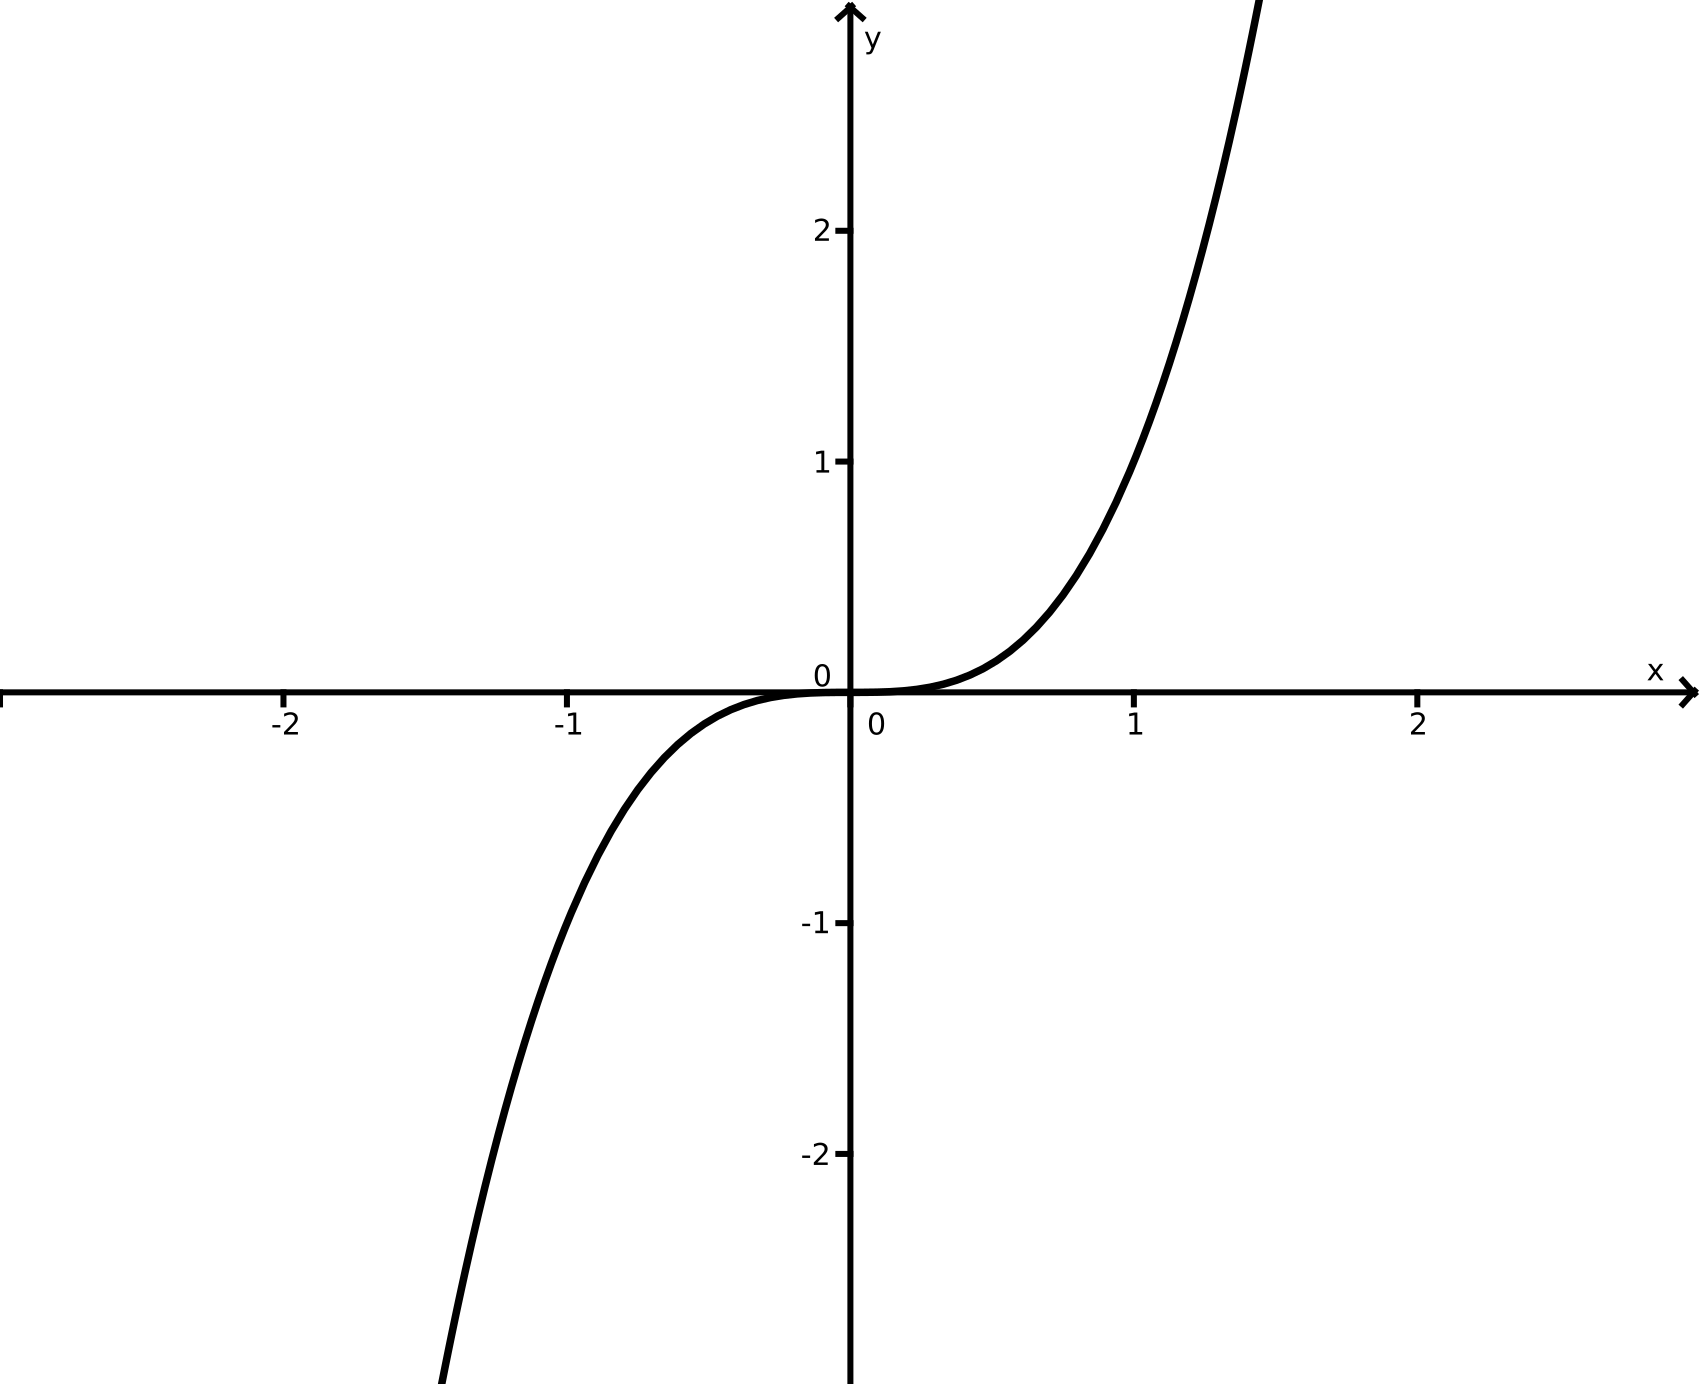
\includegraphics[scale=0.4]{img/3/1}
%  \caption{Beispiel}
%\end{figure}  

\subsection{Satz 22: Rieman}

Ist $\sum a_n$ konvergent aber nicht absolut konvergent $\implies$ Für $c \in \R$ (oder $c=+\infty$ oder $c=+\infty$) existieren Umordnungen von $\sum \alpha_n$ die gegen $c$ konvergieren!

\section{Produkt von Reihen}

\[\sum a_n, \sum b_n, \left( \sum a_n \right) \left( \sum b_n \right)\]
\[\left( \sum_{l=0}^n a_l \right) \left( \sum_{m=0}^k b_m \right) = \sum_{l=0}^n \sum_{m=0}^k a_l b_m \]


\subsection{Satz 23}

Sei $(b_{lm})_{l,m \in \N_0}$, $b_{lm} \geq 0$ und
\[S:= \sum_{l=0}^\infty \left( \sum_{m=0}^\infty b_{lm} \right) \quad (S= + \infty \text{ erlaubt!})\]

%Datei fehlt
%%\begin{figure}[!ht]
%  \centering
%    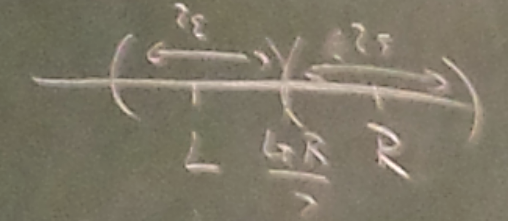
\includegraphics[scale=0.4]{img/3/2}
%  \caption{Veranschaulichung}
%\end{figure}  

\[\text{Dann ist } S:= \sum_{m=0}^\infty \left( \sum_{l=0}^\infty b_{lm} \right)\]

Ferner ist $lm$ jede Bijektion $\sigma: \N_0 \to \N_0 \times \N_0$ (d.h. für jede Abzählung von $\N_0 \times \N_0$) auch.
\[S= \sum_{n=0}^\infty b_{\sigma(n)}\]
Insbesondere kommt es auf die Reihenfolge der Summation \underline{nicht} an und z.B. gilt
\[S=\sum_{n=0}^\infty * \sum_{l+m=n} b_{lm} = \sum_{n=0}^\infty \sum_{l=0}^n b_{l,n.l}\]
\[= \lim_{L\to \infty} \sum_{l,n=0}^L b_{lm}\]

\begin{proof}

\[b_{l,m} \geq 0 \quad \forall l,m\]
\[\stackrel{\begin{array}{c}\text{Monotone}\\\text{Konvergenz}\end{array}}{\Longrightarrow} \sum_{l=0}^\infty  \left( \sum_{m=0}^\infty b_{lm} \right) \]
\[=\limN \left( \sum_{l=0}^n \left( \sum_{m=0}^\infty b_{lm} \right) \right)\]
\[=\limN \left( \sum_{l=0}^n \left( \limN[k] \sum_{m=0}^k b_{lm} \right) \right)\]
\[=\limN \left( \limN[k] \sum_{l=0}^n \sum_{m=0}^k b_{lm} \right)\]
\[=\limN \left( \limN[k] \sum_{m=0}^k \sum_{l=0}^n b_{lm} \right)\]
\[\stackrel{\begin{array}{c}\text{Monotone}\\\text{Konvergenz}\end{array}}{=}\sup_{n \in \N_0} \left( \sup_{k \in \N_0} \sum_{m=0}^k \sum_{l=0}^n b_{lm} \right)\]
\[\stackrel{\text{Lemma 24}}{=}\sup_{k \in \N_0} \left( \sup_{n \in \N_0} \sum_{m=0}^k \sum_{l=0}^n b_{lm} \right)\]
\[\stackrel{\begin{array}{c}\text{Monotone}\\\text{Konvergenz}\end{array}}{=}\limN[k] \left( \limN[n] \sum_{m=0}^k \sum_{l=0}^n b_{lm} \right)\]
\[=\ldots=\sum_{m=0}^\infty \sum_{l=0}^\infty b_{lm} \text{ \huge !}\]
Sei $\sigma: \N_0 \times \N_0$ eine Bijektion.
\[S_L = \sum_{n=1}^\infty \underbrace{b_{\sigma(n)}}_{\geq 0} \qquad  \text{\qq{Partialsumme}}\]
\[\implies S_L \leq S_{L+1} \quad \forall L \quad \& \quad \boxed{S_L \leq S}\]
Fall $ S < \infty $
\[\stackrel{\begin{array}{c}\text{Monotone}\\\text{Konvergenz}\end{array}}{\implies}\stackrel{1}{S} := \lim_{L \to \infty} S_L \text{ existiert}\]
\[\implies \sum_{n=0}^\infty b_{\sigma(n)}\]
\[\text{Damit ist } \sumNI b_{\sigma(n)} \text{ absolut konvergent}\]
\[\stackrel{\text{Satz 21}}{\implies} \text{Jede Umordnung von } \sumNI b_{\sigma(n)} \text{ konvergiert gegen } \tilde{S}\]
\[\implies \text{Für \underline{jede} Bijektion } \sigma: \N_0 \to \N_0 \times \N_0 \text{ ist } \sumNI b_{\sigma(n)} = \tilde{S}\]
Behauptung: $\tilde{S} = S$!
\[\text{Sicherlich ist } \tilde{S} \leq S, \text{ da } \tilde{S}= \lim S_L \leq S\]
\[\sum_{l=1}^{N_1} \sum_{m=1}^{N_2} b_{lm} \geq S-\epsilon\]
\[\tilde{S} \geq S-\epsilon \quad \forall \epsilon > 0\]
\[\implies \tilde{S} \geq S !\]

\end{proof}

\subsection{Lemma 24}

Seien $X,Y$ beliebige Mengen $\neq \emptyset$
\[\rho:X \times Y \to \R, \implies \sup_{x \in X} \left( \sup_{y \in Y} f(x,y) \right) = \sup_{y \in Y} \left( \sup_{x \in X} f(x,y) \right) \]

\begin{proof}

Offensichtlich
\[f(x,y) \leq \sup_{x \in X} \left( \sup_{y \in Y} f(x,y) \right)\]
Dann scharf hinschauen! %Bitches!%

\end{proof}

\subsection{Satz 25}

Sind $\sum a_n$,$\sum b_n$, \quad $a_n$, $\sum b_n \in \mathbb{C}$

absolut konvergente Reihen und setzen nun
\[\boxed{P:= \left( \sum_{n=0}^\infty a_n \right)\left( \sum_{n=0}^\infty b_n \right)} \quad (1)\]
\[\implies \boxed{P := \sum_{j=0}^\infty \left( \sum_{k=0}^\infty  a_j b_k \right) = \sum_{k=0}^\infty \left( \sum_{j=0}^\infty  a_j b_k \right)} \quad (2)\]
\[\text{ Ferner ist mit } d_{lm} = a_l b_m \text{ und jeder Bijektion:} \sigma:\N_0 \to \N_0 \times \N_0 \]
\[c_v := d_{\sigma(v)} \quad (\text{d.h. jeder Anordnung der Punkte } a_l b_m) \text{ auch }\]
\[\boxed{P= \sum_{v=0}^\infty c_v} \quad (3)\]
\[\text{und die Reihe in (3) ist absolut konvergent.}\]
\[\text{Insbesondere ist}\]
\[\boxed{P=\sum_{n=0}^\infty * \sum_{l+m=n} a_l b_n } \quad (4)\]
\[\text{als } P=\sum_{n=0}^\infty \sum_{l=0}^n a_l b_{n-l}\]
\[\text{(Cauchy Produktfornel!)}\]

\subsubsection{Bemerkung}

Satz ist falsch, falls $\sum a_n \sum b_n$ nicht absolut konvergent sind.

\begin{proof}
\[K^{'}=\sum_n |a_n|, \quad K^{''} = \sum_n |b_n|\]
\[\implies \sum_{l=0}^n \sum_{m=0}^k |a_l b_m| = \left( \sum_{l=0}^n |a_n| \right)\left( \sum_{m=0}^k |b_m| \right) \leq K^{'}K^{''} = K < \infty \]
\[\implies \sum_{l=0}^\infty \left( \sum_{m=0}^\infty |a_lb_m| \right) \leq k < \infty\]
d.h. Satz 23 kann auf $|d_{lm}=|a_lb_m|$ angewandt werden!
\[\implies \text{Jede anordnung } c_v = a_lb_m \text{ mit } (l,m) = \sigma(v), \sigma : \N_0 \to \N_0 \times \N_0 \]
\[\text{ergibt eine absolut konvergente Reihe!}\]
\[\implies \tilde{P} := \sum_{v=0}^\infty c_v \text{ existiert und ist unabhängig von } \sigma !\]
\[\implies \boxed{\tilde{P} = \sum_{n=0}^\infty * \sum_{l+m=n}} \quad !\]
\[\text{und } = \limN \sum_{l=0}^n \sum_{m=0}^n a_l b_m\]
\[= \limN \left( \sum_{l=0}^n a_l \right) \left( \sum_{m=0}^n b_m \right)\]
\[= \limN \left( \sum_{l=0}^n a_l \right) \left( \limN \sum_{m=0}^n b_m \right) \]
\[=n*v\]
\[u = \lim u_n = \limN \sum_{l=0}^n a_l\]
\[v = \lim v_n = \limN \sum_{m=0}^n b_m\]
\[\text{Da ferner } n*v = \left( \limN u_n \right)v\]
\[ = \limN (u_n*v)\]
\[ = \limN \left( \sum_{l=0}^n a_l \sum_{m=0}^\infty b_m \right) \]
\[ = \limN \sum_{l=0}^n \left( \sum_{m=0}^\infty a_lb_m \right) \]
\[ = \sum_{l=0}^\infty \left( \sum_{m=0}^\infty a_l b_m \right) \]
\[\text{und dasselbe für } u*v = \limN u*v_n\]
\[\implies \text{ (2) gilt}\]

\end{proof}

%HIER FEHLT NOCH EINE VORLESUNG!


\begin{equation}
 \begin{align}
  e = \lim_n^8 (1+\frac{1}{n})^n \\
  \tilde{e} &= \sumNI \frac{1}{n!} \\
  (1+\frac{1}{n})^n = \sum_{k=0}^n \binom {n} {k} \frac{1}{n^2} = \sum_k=0^n \frac{1}{k!} \prod_{l=0}^{k+1} \frac{n+l}{n}
 \end{align}  
\end{equation}
Wir möchten:
\begin{equation}
\begin{align}
 e = \limN (1+\frac{1}{n})^n &= \limN \sum_{k=0}^{n} \frac{1}{k!} \prod_{l=0}^{k} \frac{n-k}{k} \\
  &= \sum_{k=0}^\infty \frac{1}{k!} \limN \prod_{l=0}^{k+1} \frac{n+l}{n} \\
  &= \sum_{k=0}^\infty \frac{1}{k!}
 \end{align}
\end{equation}
Hier stellt sich die Frage, ob die zweite Zeile erlaubt ist. Bisher können wir sie nicht beweisen.
Wir benutzen folgenden Trick:

Wählen $m \in \N$
\begin{equation}
 \begin{split}
  n \ge m \\
  \implies (1 + \frac{1}{n})^n &= \sum_k=0^n \frac{1}{k!} \prod_{l=0}^{k+1} \frac{n+l}{n} \\
			      & \ge \sum_l=0^m \frac{1}{k!} \prod_{l=0}^{k+1} \frac{m+l}{m} \\
  e = \limN (1+\frac{1}{n})^n & \ge \lim_{n\to m} \sum_l=0^m \frac{1}{k!} \prod_{l=0}^{k+1} \frac{n+l}{n} \\
			      & = \sum_k=0^{m} \frac{1}{k!} \prod_{l=0}^{k+1} \lim {n \to m} \frac{n+l}{n} = \sum_{k+l}^m \frac{1}{k!} \\
  \implies e \ge \sum_{k=0}^n \frac{1}{k!} \forall m \in \N  \\
  \implies e \limN \sum_{k=0}^n \frac{1}{k!} = \sum_{k=m}^\infty \frac{1}{k!} = \tilde{e}
  \end{split}
\end{equation}

\section{Def 33:}
Für $z \in \K setzen wir:$ 
$$exp(z) = \sum_{n=0}^m = \frac{z^n}{n!}$$

Wegen des Quotientenkriteriums:
$$\left| \frac{\frac{z^{n+1}}{|n+1|!}}{\frac{z^n}{n!}} \right| = \frac{|z|}{n+1} \to 0 \text{ für } n \to \infty$$
Konvergiert absolut $\forall z \in \K$

\section{Satz 34 Eigenschaften von exp}
\begin{enumerate}
 \item $\overline{exp(z)} = exp(\overline{z})$
 \item $exp(a) + exp(b) = exp(a+b) \forall a,b \in \K$ \\
  und damit \begin{enumerate}
             \item $exp(z) \ne 0 \forall z \in \K$
             \item $exp(z)^{-1} = exp(-z)$
             \item $exp(x) >0 \forall x \in \R$
             \item Sogar $$exp(x) >1 \forall x > 0$$
            \end{enumerate}
  \item Eulersche Formeln %TODO: Herausfinden und einfügen
\end{enumerate}
Es gilt: $sin(x), cos(x) \in \R \forall x \in \R$ \\
$\left.
\begin{array}{cc} % für mehrzeiligen Text nötig
cos (-z) = cos(z) \\ sin (-z) = -sin(z) 
\end{array}
\right\}
\forall z \in \K
$

Summe der Formeln:
\begin{equation}
 \begin{split}
exp(iz) = cos(z) + i sin(z) \\
cos(z) = \frac{1}{2} (exp(iz) + exp(-iz))\\
sin(z) &= \frac{1}{2e} (exp(iz) - exp(-iz))\\
\implies (cos(z))^2 + (sin(z))^2 = 1 \forall z \in \K \\
Re(exp(ix)) = cos(x) \\
Im(exp(ix)) = sin(x) \\
|exp(ix) \ge 1| \\
|cos(x)| , |sin(x) \le 1
 \end{split}
\end{equation}

%TODO: Beweise einfügen






